\documentclass[
    twocolumn,
    fontsize = 10pt,
    parskip = half+,
    headings = small,
    headwidth = text,
    footwidth = text,
]{scrartcl}

\usepackage{pdflscape}
\usepackage{pgfgantt}
\usepackage{pdflscape}
\usetikzlibrary{shapes,backgrounds, arrows, positioning, trees, shadows}
\usepackage{pgf}
\usepackage{pgfplots}
\pgfplotsset{compat=1.18}
\selectcolormodel{rgb}

\KOMAoptions{
 paper = A4,
 pagesize,
 % headlines = 1.1,
 % headsepline,
 DIV = calc,
}
\typearea{11}

%\usepackage{fontspec}
%\setmainfont{Roboto Condensed}

\usepackage[
  todonotes={textsize=footnotesize},
  commandnameprefix=ifneeded,
  ulem={normalem,normalbf}
]{changes}
\definechangesauthor[name={Khalil Ben Larbi}, color=green]{kbl}

\usepackage{amsmath}

\usepackage[
  detect-all
]{siunitx}

\usepackage[
  style = ieee,
  backend = biber,
  hyperref = true,
  backref = true,
  seconds = true,
  date = iso,
]{biblatex}

\addbibresource{bib/bibliography.bib}

\usepackage{xurl}

\usepackage[acronyms=true]{glossaries}

\usepackage[
    colorlinks=true,
    allcolors=,
]{hyperref}

\usepackage[
    capitalize,
    nameinlink,
    noabbrev,
]{cleveref}

\newcommand{\rftvector}[1]{\underline{#1}}
\newcommand{\rftmatrix}[1]{\underline{\underline{#1}}}
\newcommand{\rftquaternion}[1]{\boldsymbol{#1}}

\newacronym{dfg}{DFG}{Deutsche Forschungsgemeinschaft}

\newacronym{rfi}{RFI}{Chair of Space Informatics and Satellite Systems}
\newacronym{rtg}{RTG}{radioisotope thermoelectric generator}

\newacronym{jmu}{JMU}{Julius-Maximilians-Universität Würzburg}

\newglossaryentry{cubesat}{
    name = CubeSat,
    description = {A small satellite following the form factor defined by the CubeSat Design Specification}
}

\makeglossaries

\title{Firmware for Gecko Testbed: Applications in Capturing Orbital Debris}
% \subtitle{Turning Humans into Space Scientists since 2003}
\author{
    \begin{minipage}[t]{.8\textwidth}
        \centering
         Ateeb Ahmed, Roshan Kumar Gupta, Vassilios Papadopoulos
    \end{minipage}
}
\date{August 20, 2025}

\begin{document}
\twocolumn[
\begin{@twocolumnfalse}

\maketitle

\begin{abstract}
Following the title, the abstract is the \textbf{second} most frequently read part of a scientific paper.
It informs about the general content and determines the paper's relevance for the reader.
It is good practice to write the abstract when writing the paper is \textbf{finished} in a way that it condenses and summarizes the content of the paper.
Only start writing the abstract when all required research and work has been finished.
Make the abstract one paragraph without reference and use about \numrange{200}{500} words.
Be sure to only draw conclusions and make only statements that are included in the paper.
Keep the text of the abstract in present tense.
A good approach to drafting an abstract is to start by summarizing  each section of the paper in \numrange{1}{2} sentences.
\end{abstract}
\end{@twocolumnfalse}
]


%------------------------------------------------------------------------------	
%------------------------------------------------------------------------------	
\section{Introduction}
%------------------------------------------------------------------------------
In the last century mankind has made unprecedented technological advances and discoveries. Naturally, Space exploration, which has fascinated all civilizations that have existed, also had a breakthrough in the previous century when USA launched Apollo 11 on 26th July 1969 to Moon. While this project was mainly targeted to explore the lunar surface. Since then many other such objects are sent in space but only to perform specific tasks like communication, observation and scientific research. These objects usually orbit around Earth and are called Satellite. 
Currently, there are 7,560 satellites orbiting Earth \cite{ucs}. But keeping these satellites operational require constant maintainance since they are exposed to extreme temperatures, radiation and micro-meteoroids. Unfortunately, not all satellites stay operational through out their mission and gracefully leave the orbit. Some gets destroyed during deployment, or lose contact and control from Earth due to communication issues. These dead satellites and other small objects created due to some form of damage to existing satellites are collectively called "Space Debris". 
There are currently 32,750 cataloged and tracked debris objects, these 50 cm or more in size and traveling at a speed of 3 km/s \cite{space_junk}. \\

These objects also travel with a random trajectory and are not predictable. Collision with this debris can be fatal for not only existing operational satellites but also for future deployments. To this end, ClearSpace SA, a Swiss startup, is developing a device resembling a four-armed "space claw" that would grip junk satellites and de-orbit them. The project is expected to go live in late 2029, and intends to de-orbit a special kind of space debris called VESPA (Vega Secondary Payload Adapter) \cite{clear_space}. 

Recently, Gecko materials have shown promise in catching space debris [link]. Gecko materials exhibits certain properties which are desirable in space debris collection, such as: Gecko materials only require smooth surfaces. Gecko Materials do not require adhesive substance and work purely through fundamental property of materials called Van Der Waals forces. Due to these properties Gecko materials offer multiple docking opportunities to any space debris and offer good re-usability.

Given promising results from early proof of concept studies on Gecko materials for space debris collection, further research on how gecko materials behave in space-like conditions such as a combination of extreme temperatures, radiation, vaccume and microgravity is needed. 

In this regard, TU Berlin and Julius-Maximilian-Universität Würzburg as part of the \textbf{gEICko: GEcko based Innovative Capture Kit for uncooperative and unprepared Orbital assets} has initiated a joint investigation of Gecko materials. The team from TU Berlin has developed a Testbed. The goal of this Testbed is to compare different kinds of gecko materials against each other. The testbed is also suitable for simulated space-like environments since it is robust and vacuum sealed, a more detailed description of TestBed is provided in the following section.

This project, in particular, is concerned with developing a firmware to control the testbed and provide researchers with an intuitive but exhaustive user interface (UI) to be able to command and control this testbed.

\subsection{The Gecko Testbed}

\begin{figure}[h]
    \centering
    \includegraphics[width=1.0\linewidth]{pics/gecko_testbed.png}
    \caption{Testbed to test Gecko materials.}
    \label{fig: gecko testbed}
\end{figure}

Figure 1 shows an image of the testbed developed by the engineers from TU Berlin. This consists of 3 stepper motors. Each motor is responsible for movement in each direction i.e. x, y and z axes. In this center of the testbed is a smooth glass surface which simulates a smooth surface from that of a space debris and also serves as a rendezvous point aka point of contact. The small green piece directly on top of this surface represents the Gecko material being tested. The vertical motors (z-axis) moves the Gecko material up and down along its axis and press it against the smooth surface such that the gecko material stick to it.

There is also a small 3 dimensional force sensor right underneath the smooth surface which can sense press/pull forces as well as shear and translatory forces. 

The following are the exact specifications and details of each component of the Testbed:

\begin{itemize}
    \item Stepper Motor: 3 stepper motors are used in this testbed. Each stepper motor is controlled using CL57T driver.
    \item Force Sensor: We have used a Strain Guage Force Sensor by ME Systeme model K3D40 (10N). We have further used GSV-4USB amplifier to control force sensor and also to serialize the output.
    \item Power Supply: We have used a generic powersupply easily available in all labs at 24V and 1.5A.
    \item Computing Unit: We have used a Raspberry Pi micro-controller as our main computing device.
\end{itemize}

All of the components of the testbed mentioned above are shown in figure 2.

\begin{figure}[h]
    \centering
    \includegraphics[width=1.0\linewidth]{pics/gecko_testbed_components.png}
    \caption{Individual Components of Gecko Testbed.}
    \label{fig: gecko testbed components}
\end{figure}


\subsubsection{Uses Cases of Testbed}
The main purpose for this testbed is to test and compare different gecko materials in space-like environments. The metric used to measure the effectiveness of a gecko material is the ratio between push and pull force generated, then an ideal Gecko material candidate would be one which requires minimum push forces against a smooth surface, sticks to it and then can pull the stuck surface with a much higher pull force.

This testbed accomplish this by pressing the gecko material against the smooth the surface until a target push force is reached (establishing docking), and then pull away the gecko material and measuring the pull force generated by gecko material. This simple experiment can have two further possibilities: 

\begin{itemize}
    \item Case 1: When smooth surface is static and only gecko material moves up and down.
    \item Case 2: When smooth surface is static until point of contact (docking), and while gecko material start pulling the smooth surface also moves along one or both horizontal axes (X and Y).
    \item Case 3: When the gecko materials establishes contact while smooth surface is moving along horizontal axes. Similarly, pull force is also measured with gecko and smooth surface moving. This case is the most complicated out of all above and accurately simulates the behavior of uncontrolled space debris.
\end{itemize}

Now that the use cases of the testbed are laid out, in the later sections we will describe how the developed firmware handles these situations. 



%------------------------------------------------------------------------------	
\section{Methods}
%------------------------------------------------------------------------------	

%------------------------------------------------------------------------------	
\section{Results}
%------------------------------------------------------------------------------	


%------------------------------------------------------------------------------	
\section{Discussion}
%------------------------------------------------------------------------------	


%------------------------------------------------------------------------------	
\section{Conclusion}
%------------------------------------------------------------------------------	

\printbibliography

\printglossaries
% Appendix
\appendix
\pagenumbering{roman}
% Manage your appendix
% use \input{appendix/tex_file_name} to add to the appendix

% Project management
\pagebreak
\onecolumn
\begin{landscape}
\section{Project Management}
%______________________________________________________________
% Work Breakdown Structure
% Breakdown of the tasks in individual work packages.
% Up to two levels of workpackages
%______________________________________________________________

\subsection{Work Breakdown Structure}

    \small
    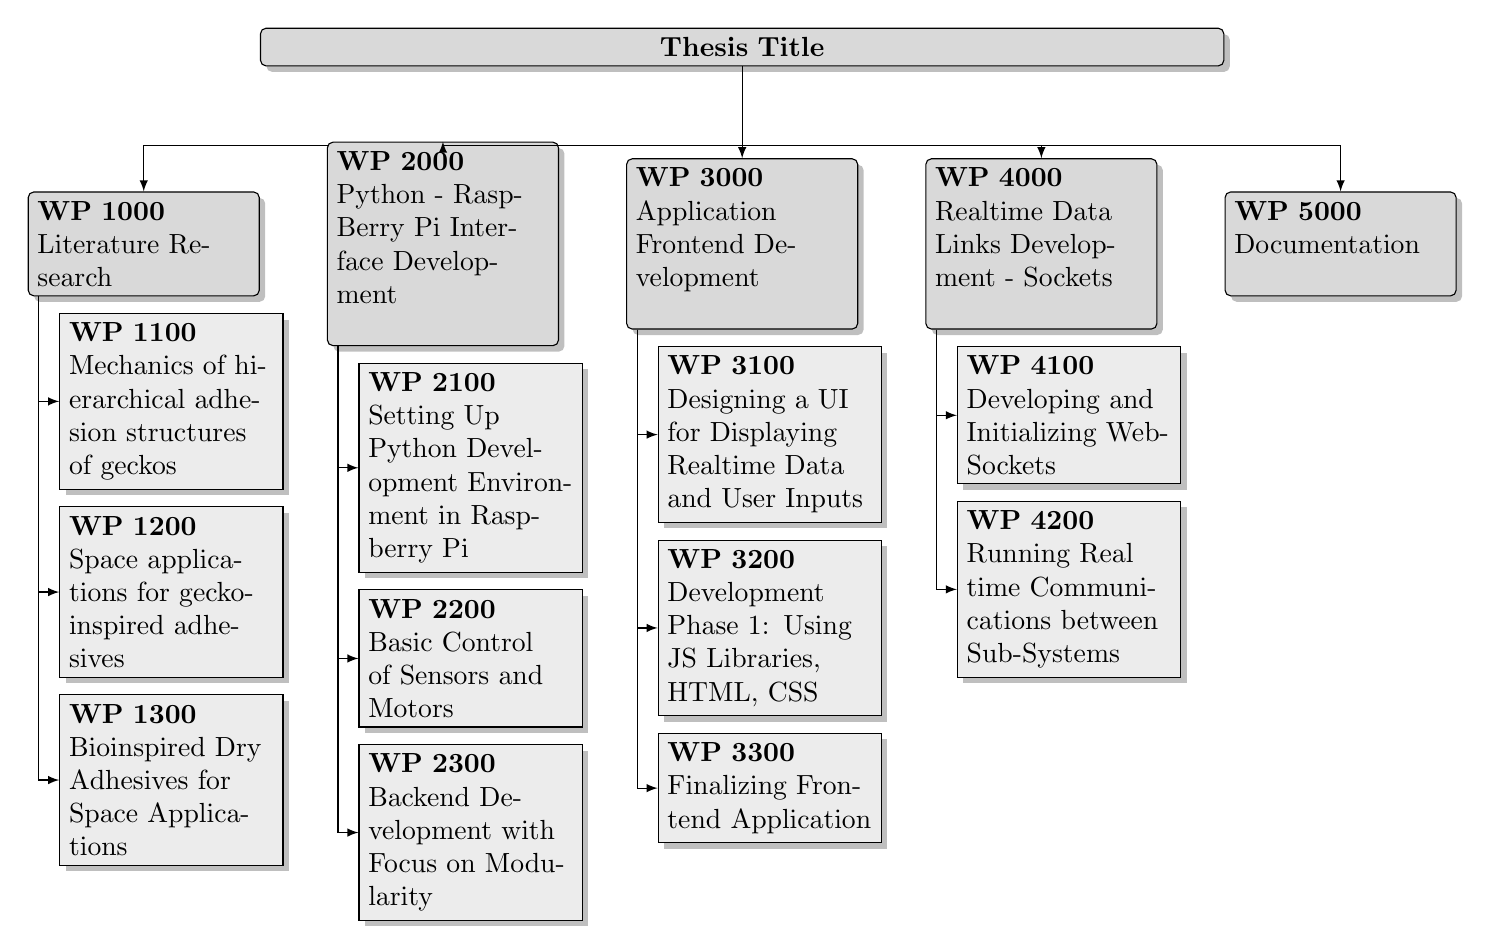
\begin{tikzpicture}[
        basic/.style   = {draw, text width=2.7cm, align=left, drop shadow, rectangle},
        root/.style    = {basic, text width=12cm, rounded corners=2pt, thin, align=center, fill=gray!30},
        level 2/.style = {basic, rounded corners=2pt, thin, fill=gray!30},
        level 3/.style = {basic, thin, fill=gray!15, text width=2.6cm},
        level 1/.style={sibling distance=38mm}, edge from parent fork down,
        edge from parent/.style={->,draw}, level distance=2.5cm,  >=latex]

    % root of the the initial tree, level 1
    \node[root] {\textbf{Thesis Title}}
    % The first level, as children of the initial tree
        child {node[level 2] (c1) {\textbf{WP~1000} \\ Literature Research}}
        child {node[level 2] (c2) {\textbf{WP~2000} \\ Python - RaspBerry Pi Interface Development \\ $~~$}}
        child {node[level 2] (c3) {\textbf{WP~3000} \\ Application Frontend Development \\ $~~$}}
        child {node[level 2] (c4) {\textbf{WP~4000} \\ Realtime Data Links Development - Sockets \\ $~~$}}
        child {node[level 2] (c5) {\textbf{WP~5000} \\ Documentation \\ $~~$}};

    % The second level, relatively positioned nodes
    \begin{scope}[every node/.style={level 3}, node distance=6pt]
    \node [below=of c1, xshift=10pt] (c11) {\textbf{WP~1100} \\ Mechanics of hierarchical adhesion structures of geckos};
    \node [below=of c11] (c12) {\textbf{WP~1200} \\ Space applications for gecko-inspired adhesives};
    \node [below=of c12] (c13) {\textbf{WP~1300} \\ Bioinspired Dry Adhesives for Space Applications};

    \node [below=of c2, xshift=10pt] (c21) {\textbf{WP~2100} \\ Setting Up Python Development Environment in Raspberry Pi };
    \node [below=of c21] (c22) {\textbf{WP~2200} \\ Basic Control of Sensors and Motors };
    \node [below=of c22] (c23) {\textbf{WP~2300} \\ Backend Development with Focus on Modularity };

    \node [below=of c3, xshift=10pt] (c31) {\textbf{WP~3100} \\ Designing a UI for Displaying Realtime Data and User Inputs};
    \node [below=of c31] (c32) {\textbf{WP~3200} \\ Development Phase 1: Using JS Libraries, HTML, CSS};
    \node [below=of c32] (c33) {\textbf{WP~3300} \\ Finalizing Frontend Application};
    % \node [below=of c33] (c34) {\textbf{WP~3400} \\ } ;

    \node [below=of c4, xshift=10pt] (c41) {\textbf{WP~4100} \\ Developing and Initializing Web-Sockets};
    \node [below=of c41] (c42) {\textbf{WP~4200} \\ Running Real time Communications between Sub-Systems};

    \end{scope}

    % lines from each level 1 node to every one of its "children"
    \foreach \value in {1,2,3}
        \draw[->] ([xshift=4pt]c1.south west) |- (c1\value.west);

    \foreach \value in {1,2,3}
        \draw[->] ([xshift=4pt]c2.south west) |- (c2\value.west);

    \foreach \value in {1,2,3}
        \draw[->] ([xshift=4pt]c3.south west) |- (c3\value.west);

    \foreach \value in {1,2}
        \draw[->] ([xshift=4pt]c4.south west) |- (c4\value.west);

    \end{tikzpicture}
    \normalsize

\end{landscape}

\begin{landscape}

%______________________________________________________________
% Gantt Chart
% Time line of the project
% Shows duration and chronological structure for each 
%  workpackage and project milestones
%______________________________________________________________
\subsection{Gantt Chart}
\definecolor{color_bar}{RGB}{0, 63, 137}
\definecolor{color_group}{RGB}{0, 37, 82}
\begin{center}
    \begin{ganttchart}[
        expand chart=.95\linewidth,
        vgrid,
        bar/.append style={fill=color_bar, draw=none},
        group/.append style={fill=color_group},
        group left shift=0,
        group right shift=0,
        group peaks tip position=0,
        group peaks height=.25,
        y unit chart = 0.445cm,
        group top shift=0.25,
        bar top shift=-0.1,
        bar height=0.6,
        milestone top shift=-0.1,
        milestone/.append style={xscale=0.5}]{1}{16}
        \gantttitle{Weeks}{16} \\
        \gantttitlelist{1,...,16}{1} \\

        \ganttgroup{WP 1000: Literature Research}{1}{5} \\
        \ganttbar{Mechanics of hierarchical adhesion structures of geckos}{1}{3} \\
        \ganttbar{Space applications for Gecko inspired adhesives}{2}{4} \\
        \ganttbar{Bioinspired Dry Adhesives for Space Applications}{2}{5} \\
        \\
        \ganttgroup{Python - RaspBerry Pi Interface
                    Development}{4}{9} \\
        \ganttbar{Setting Up Python Development Environment in Raspberry Pi}{4}{5} \\

        \ganttbar{Basic Control of Sensors and Motors}{5}{7} \\
                            
        \ganttbar{Backend Development with Focus on Modularity}{7}{9} \\
        
        \ganttmilestone{Preliminary Design Review}{9} \\
        \\
        \ganttgroup{Application Frontend Development}{4}{11} \\
        \ganttbar{Designing a UI
            for Displaying
            Realtime Data
            and User Inputs}{4}{5} \\
        \ganttbar{Developement
            Phase 1: Using JS Libraries,
            HTML, CSS}{5}{8} \\
            \ganttbar{Finalizing Frontend Application}{8}{10} \\
        \ganttmilestone{Critical Design Review}{11} \\
        \\
        \ganttgroup{Realtime Data
    Links Development - Sockets}{10}{12} \\
        \ganttbar{Developing and
    Initializing Web-Sockets}{10}{11} \\
        \ganttbar{Running Real
    time Communications between
    Sub-Systems}{11}{12} \\
        \ganttmilestone{Final Presentation}{12} \\
        \\
        \ganttgroup{WP 5000: Documentation}{1}{16} \\
        \ganttmilestone{Draft}{12} \\
        \ganttmilestone{Submission}{16}
    \end{ganttchart}
\end{center}
\end{landscape}

%______________________________________________________________
% Work Package Description
% Detailed description of each workpackage
%______________________________________________________________

\subsection{Work Package Description}

\newcommand{\wpddate}{}
%%%%
% WP1000 - Literature Research
%%%%

\begin{table}[!h]
    \begin{center}
        \begin{tabular}{|p{.2\columnwidth}||p{.3\columnwidth}|p{.27\columnwidth}||p{.23\columnwidth}|}
            \hline
            \multicolumn{3}{|l||}{\textbf{}} & \multicolumn{1}{c|}{}\\
            \multicolumn{3}{|l||}{\textbf{}} & \multicolumn{1}{c|}{\textbf{WP 1100}}\\
            \multicolumn{3}{|l||}{\textbf{}} & \multicolumn{1}{c|}{}\\
            \hline\hline
            \textbf{Title} & \multicolumn{2}{p{.40\columnwidth}||}{\textbf{Mechanics of Hierarchical Adhesion Structures of Geckos}}
            & \textbf{Page:} 1 of 1\\
            \hline
            \textbf{Responsible} & \multicolumn{2}{l||}{Roshan, Ateeb, Vassili} & \textbf{Version:} 1.0\\
            \hline
            \multicolumn{3}{|l||}{} & \textbf{Date: 21.04.2025} \\
            \hline\hline
            \textbf{Start} & \multicolumn{2}{l||}{Week 1} & \\
            \hline
            \textbf{End} & \multicolumn{2}{l||}{Week 3} & \textbf{Duration}: 1 Weeks\\
            \hline\hline
            \textbf{Processed by} & \multicolumn{3}{l|}{Roshan Kumar Gupta}\\
            \hline\hline
            \multicolumn{4}{|p{.95\columnwidth}|}{\textbf{Goals:}}\\
            \multicolumn{4}{|p{.95\columnwidth}|}{$\bullet$ Investigate bioinspired dry adhesives for space use}\\
            \multicolumn{4}{|p{.95\columnwidth}|}{$\bullet$ Optimize testbed for hierarchical adhesion analysis}\\
            \multicolumn{4}{|p{.95\columnwidth}|}{}\\
            \multicolumn{4}{|p{.95\columnwidth}|}{\textbf{Input:}}\\
            \multicolumn{4}{|p{.95\columnwidth}|}{$\bullet$ Journal papers on bioinspired dry adhesives}\\
            \multicolumn{4}{|p{.95\columnwidth}|}{$\bullet$ Conference papers on gecko adhesion structures}\\
            \multicolumn{4}{|p{.95\columnwidth}|}{}\\
            \multicolumn{4}{|p{.95\columnwidth}|}{\textbf{Connections to other WPs:}}\\
            \multicolumn{4}{|p{.95\columnwidth}|}{$\bullet$ Collaboration with TU Berlin and Fraunhofer team}\\
            \multicolumn{4}{|p{.95\columnwidth}|}{\textbf{Tasks:}}\\
            \multicolumn{4}{|p{.95\columnwidth}|}{$\bullet$ Literature research on mechanics of hierarchical adhesion structures of geckos}\\
            \multicolumn{4}{|p{.95\columnwidth}|}{}\\
            \multicolumn{4}{|p{.95\columnwidth}|}{\textbf{Results:}}\\
            \multicolumn{4}{|p{.95\columnwidth}|}{$\bullet$ Basic knowledge about mechanics of hierarchical adhesion structures of geckos}\\
            \multicolumn{4}{|p{.95\columnwidth}|}{$\bullet$ Deeper knowledge about mechanics of hierarchical adhesion structures of geckos}\\
            \hline
        \end{tabular}
    \end{center}
\end{table}

\clearpage

\begin{table}[!h]
    \begin{center}
        \begin{tabular}{|p{.2\columnwidth}||p{.3\columnwidth}|p{.27\columnwidth}||p{.23\columnwidth}|}
            \hline
            \multicolumn{3}{|l||}{\textbf{}} & \multicolumn{1}{c|}{}\\
            \multicolumn{3}{|l||}{\textbf{}} & \multicolumn{1}{c|}{\textbf{WP 1200}}\\
            \multicolumn{3}{|l||}{\textbf{}} & \multicolumn{1}{c|}{}\\
            \hline\hline
            \textbf{Title} & \multicolumn{2}{p{.40\columnwidth}||}{\textbf{Space Applications for Gecko-Inspired Adhesives}}
            & \textbf{Page:} 1 of 2\\
            \hline
            \textbf{Responsible} & \multicolumn{2}{l||}{Ateeb, Roshan, Vassili} & \textbf{Version:} 1.0\\
            \hline
            \multicolumn{3}{|l||}{} & \textbf{Date:28.04.2025} \\
            \hline\hline
            \textbf{Start} & \multicolumn{2}{l||}{Week 2} & \\
            \hline
            \textbf{End} & \multicolumn{2}{l||}{Week 4} & \textbf{Duration}: 1 Weeks\\
            \hline\hline
            \textbf{Processed by} & \multicolumn{3}{l|}{Ateeb, Roshan, Vassili}\\
            \hline\hline
            \multicolumn{4}{|p{.95\columnwidth}|}{\textbf{Goals:}}\\
            \multicolumn{4}{|p{.95\columnwidth}|}{$\bullet$ Investigate space applications of gecko-inspired adhesives}\\
            \multicolumn{4}{|p{.95\columnwidth}|}{$\bullet$ Optimize testbed for space-relevant adhesion analysis}\\
            \multicolumn{4}{|p{.95\columnwidth}|}{}\\
            \multicolumn{4}{|p{.95\columnwidth}|}{\textbf{Input:}}\\
            \multicolumn{4}{|p{.95\columnwidth}|}{$\bullet$ Journal papers on gecko-inspired adhesives}\\
            \multicolumn{4}{|p{.95\columnwidth}|}{$\bullet$ Conference papers on space applications of adhesives}\\
            \multicolumn{4}{|p{.95\columnwidth}|}{}\\
            \multicolumn{4}{|p{.95\columnwidth}|}{\textbf{Connections to other WPs:}}\\
            \multicolumn{4}{|p{.95\columnwidth}|}{$bullet$ Collaboration with TU Berlin and Fraunhofer team}\\
            \multicolumn{4}{|p{.95\columnwidth}|}{\textbf{Tasks:}}\\
            \multicolumn{4}{|p{.95\columnwidth}|}{$\bullet$ Literature research on space applications for gecko-inspired adhesives}\\
            \multicolumn{4}{|p{.95\columnwidth}|}{}\\
            \multicolumn{4}{|p{.95\columnwidth}|}{\textbf{Results:}}\\
            \multicolumn{4}{|p{.95\columnwidth}|}{$\bullet$ Basic knowledge about space applications for gecko-inspired adhesives}\\
            \multicolumn{4}{|p{.95\columnwidth}|}{$\bullet$ Deeper knowledge about space applications for gecko-inspired adhesives}\\
            \hline
        \end{tabular}
    \end{center}
\end{table}

\clearpage

\begin{table}[!h]
    \begin{center}
        \begin{tabular}{|p{.2\columnwidth}||p{.3\columnwidth}|p{.27\columnwidth}||p{.23\columnwidth}|}
            \hline
            \multicolumn{3}{|l||}{\textbf{}} & \multicolumn{1}{c|}{}\\
            \multicolumn{3}{|l||}{\textbf{}} & \multicolumn{1}{c|}{\textbf{WP 1300}}\\
            \multicolumn{3}{|l||}{\textbf{}} & \multicolumn{1}{c|}{}\\
            \hline\hline
            \textbf{Title} & \multicolumn{2}{p{.40\columnwidth}||}{\textbf{Bioinspired Dry Adhesives for Space Applications}}
            & \textbf{Page:} 1 of 3\\
            \hline
            \textbf{Responsible} & \multicolumn{2}{l||}{Ateeb, Roshan, Vassili} & \textbf{Version:} 1.0\\
            \hline
            \multicolumn{3}{|l||}{} & \textbf{Date: 05.05.2025} \wpddate\\
            \hline\hline
            \textbf{Start} & \multicolumn{2}{l||}{Week 2} & \\
            \hline
            \textbf{End} & \multicolumn{2}{l||}{Week 5} & \textbf{Duration}: 4 Weeks\\
            \hline\hline
            \textbf{Processed by} & \multicolumn{3}{l|}{Ateeb, Roshan, Vassili}\\
            \hline\hline
            \multicolumn{4}{|p{.95\columnwidth}|}{\textbf{Goals:}}\\
            \multicolumn{4}{|p{.95\columnwidth}|}{$\bullet$ Investigate bioinspired dry adhesives for space use}\\
            \multicolumn{4}{|p{.95\columnwidth}|}{$\bullet$ }\\
            \multicolumn{4}{|p{.95\columnwidth}|}{}\\
            \multicolumn{4}{|p{.95\columnwidth}|}{\textbf{Input:}}\\
            \multicolumn{4}{|p{.95\columnwidth}|}{$\bullet$ Documentation of literature topic 3}\\
            \multicolumn{4}{|p{.95\columnwidth}|}{}\\
            \multicolumn{4}{|p{.95\columnwidth}|}{\textbf{Connections to other WPs:}}\\
            \multicolumn{4}{|p{.95\columnwidth}|}{$\bullet$ \textbf{WP 3200} Research for subsystems/units/parts/components}\\
            \multicolumn{4}{|p{.95\columnwidth}|}{$\bullet$ \textbf{WP 3200} Gather technical solutions for novel design}\\
            \multicolumn{4}{|p{.95\columnwidth}|}{}\\
            \multicolumn{4}{|p{.95\columnwidth}|}{\textbf{Tasks:}}\\
            \multicolumn{4}{|p{.95\columnwidth}|}{$\bullet$ Literature research on literature topic 3}\\            \multicolumn{4}{|p{.95\columnwidth}|}{}\\
            \multicolumn{4}{|p{.95\columnwidth}|}{\textbf{Results:}}\\
            \multicolumn{4}{|p{.95\columnwidth}|}{$\bullet$ Select technical solutions of literature topic 3 as proposal for thingy to be developed}\\
            \hline
        \end{tabular}
    \end{center}
\end{table}

\clearpage

%%%%
% WP2000 - Main Task 1
%%%%

\begin{table}[!h]
    \begin{center}
        \begin{tabular}{|p{.2\columnwidth}||p{.3\columnwidth}|p{.27\columnwidth}||p{.23\columnwidth}|}
            \hline
            \multicolumn{3}{|l||}{\textbf{}} & \multicolumn{1}{c|}{}\\
            \multicolumn{3}{|l||}{\textbf{}} & \multicolumn{1}{c|}{\textbf{WP 2100}}\\
            \multicolumn{3}{|l||}{\textbf{}} & \multicolumn{1}{c|}{}\\
            \hline\hline
            \textbf{Title} & \multicolumn{2}{p{.40\columnwidth}||}{\textbf{Setting Up
Python Development Environment in Raspberry Pi}}
            & \textbf{Page:} 1 of 1\\
            \hline
            \textbf{Responsible} & \multicolumn{2}{l||}{Ateeb, Roshan, Vassili} & \textbf{Version:} 1.0\\
            \hline
            \multicolumn{3}{|l||}{} & \textbf{Date: } 19.05.2025 \\
            \hline\hline
            \textbf{Start} & \multicolumn{2}{l||}{Week 4} & \\
            \hline
            \textbf{End} & \multicolumn{2}{l||}{Week 5} & \textbf{Duration}: 1 Week\\
            \hline\hline
            \textbf{Processed by} & \multicolumn{3}{l|}{Ateeb, Roshan, Vassili}\\
            \hline\hline
            \multicolumn{4}{|p{.95\columnwidth}|}{\textbf{Goals:}}\\
            \multicolumn{4}{|p{.95\columnwidth}|}{$\bullet$ Setup development environment including Github, Visual Studio IDE and SSH for remote access.}\\

            \multicolumn{4}{|p{.95\columnwidth}|}{}\\
            \multicolumn{4}{|p{.95\columnwidth}|}{\textbf{Input:}}\\
            \multicolumn{4}{|p{.95\columnwidth}|}{$\bullet$ None }\\

            \multicolumn{4}{|p{.95\columnwidth}|}{}\\
            \multicolumn{4}{|p{.95\columnwidth}|}{\textbf{Connections to other WPs:}}\\
            \multicolumn{4}{|p{.95\columnwidth}|}{$\bullet$ This is a base WP, other WPs are dependent on this.}\\
            \multicolumn{4}{|p{.95\columnwidth}|}{}\\
            \multicolumn{4}{|p{.95\columnwidth}|}{\textbf{Tasks:}}\\
            \multicolumn{4}{|p{.95\columnwidth}|}{$\bullet$ Same as in goals}\\
            \multicolumn{4}{|p{.95\columnwidth}|}{}\\
            \multicolumn{4}{|p{.95\columnwidth}|}{\textbf{Results:}}\\
            \multicolumn{4}{|p{.95\columnwidth}|}{$\bullet$ An environment is setup which enables contributors to start working.}\\
            \hline
        \end{tabular}
    \end{center}
\end{table}

\clearpage

\begin{table}[!h]
    \begin{center}
        \begin{tabular}{|p{.2\columnwidth}||p{.3\columnwidth}|p{.27\columnwidth}||p{.23\columnwidth}|}
            \hline
            \multicolumn{3}{|l||}{\textbf{}} & \multicolumn{1}{c|}{}\\
            \multicolumn{3}{|l||}{\textbf{}} & \multicolumn{1}{c|}{\textbf{WP 2200}}\\
            \multicolumn{3}{|l||}{\textbf{}} & \multicolumn{1}{c|}{}\\
            \hline\hline
            \textbf{Title} & \multicolumn{2}{p{.40\columnwidth}||}{\textbf{Basic Control of Sensors and Motors}}
            & \textbf{Page:} 1 of 1\\
            \hline
            \textbf{Responsible} & \multicolumn{2}{l||}{Ateeb, Roshan, Vassili} & \textbf{Version:} 1.0\\
            \hline
            \multicolumn{3}{|l||}{} & \textbf{Date:} 26.05.2025 \\
            \hline\hline
            \textbf{Start} & \multicolumn{2}{l||}{Week 5} & \\
            \hline
            \textbf{End} & \multicolumn{2}{l||}{Week 7} & \textbf{Duration}: 3 Weeks\\
            \hline\hline
            \textbf{Processed by} & \multicolumn{3}{l|}{Ateeb, Roshan, Vassili}\\
            \hline\hline
            \multicolumn{4}{|p{.95\columnwidth}|}{\textbf{Goals:}}\\
            \multicolumn{4}{|p{.95\columnwidth}|}{$\bullet$ Motors and Sensors are controlled through Python Interface}\\
            \multicolumn{4}{|p{.95\columnwidth}|}{}\\
            \multicolumn{4}{|p{.95\columnwidth}|}{\textbf{Input:}}\\
            \multicolumn{4}{|p{.95\columnwidth}|}{$\bullet$ Results from WP 2100}\\
            \multicolumn{4}{|p{.95\columnwidth}|}{}\\
            \multicolumn{4}{|p{.95\columnwidth}|}{\textbf{Connections to other WPs:}}\\
            \multicolumn{4}{|p{.95\columnwidth}|}{$\bullet$ Future WPs depend on this. Since we are working serially.}\\
            \multicolumn{4}{|p{.95\columnwidth}|}{}\\
            \multicolumn{4}{|p{.95\columnwidth}|}{\textbf{Tasks:}}\\
            \multicolumn{4}{|p{.95\columnwidth}|}{$\bullet$ Produce Code which can control motors and sensors of testbed when executed.}\\
            \multicolumn{4}{|p{.95\columnwidth}|}{}\\
            \multicolumn{4}{|p{.95\columnwidth}|}{\textbf{Results:}}\\
            \multicolumn{4}{|p{.95\columnwidth}|}{$\bullet$ Yet to be worked on.}\\
            \hline
        \end{tabular}
    \end{center}
\end{table}

\clearpage

\begin{table}[!h]
    \begin{center}
        \begin{tabular}{|p{.2\columnwidth}||p{.3\columnwidth}|p{.27\columnwidth}||p{.23\columnwidth}|}
            \hline
            \multicolumn{3}{|l||}{\textbf{}} & \multicolumn{1}{c|}{}\\
            \multicolumn{3}{|l||}{\textbf{}} & \multicolumn{1}{c|}{\textbf{WP 2300}}\\
            \multicolumn{3}{|l||}{\textbf{}} & \multicolumn{1}{c|}{}\\
            \hline\hline
            \textbf{Title} & \multicolumn{2}{p{.40\columnwidth}||}{\textbf{Backend Development with Focus on Modularity}}
            & \textbf{Page:} 1 of 1\\
            \hline
            \textbf{Responsible} & \multicolumn{2}{l||}{Ateeb, Roshan, Vassili} & \textbf{Version:} 1.0\\
            \hline
            \multicolumn{3}{|l||}{} & \textbf{Date:} 10.06.2025 \\
            \hline\hline
            \textbf{Start} & \multicolumn{2}{l||}{Week 7} & \\
            \hline
            \textbf{End} & \multicolumn{2}{l||}{Week 9} & \textbf{Duration}: 2 Weeks\\
            \hline\hline
            \textbf{Processed by} & \multicolumn{3}{l|}{Ateeb, Roshan, Vassili}\\
            \hline\hline
            \multicolumn{4}{|p{.95\columnwidth}|}{\textbf{Goals:}}\\
            \multicolumn{4}{|p{.95\columnwidth}|}{$\bullet$ A fully fledged, modular Backend framework for controlling all components of TestBed}\\
            \multicolumn{4}{|p{.95\columnwidth}|}{}\\
            \multicolumn{4}{|p{.95\columnwidth}|}{\textbf{Input:}}\\
            \multicolumn{4}{|p{.95\columnwidth}|}{$\bullet$ Results from WP2200 are extended here.}\\
            \multicolumn{4}{|p{.95\columnwidth}|}{}\\
            \multicolumn{4}{|p{.95\columnwidth}|}{\textbf{Connections to other WPs:}}\\
            \multicolumn{4}{|p{.95\columnwidth}|}{}\\
            \multicolumn{4}{|p{.95\columnwidth}|}{\textbf{Tasks:}}\\
            \multicolumn{4}{|p{.95\columnwidth}|}{$\bullet$ Write a framework-like which controls all sensors and motors of testbed.}\\
            \multicolumn{4}{|p{.95\columnwidth}|}{$\bullet$ Make sure the application is modular and testbed modules can be swapped with no effect on working of application}\\
            \multicolumn{4}{|p{.95\columnwidth}|}{}\\
            \multicolumn{4}{|p{.95\columnwidth}|}{\textbf{Results:}}\\
            \multicolumn{4}{|p{.95\columnwidth}|}{$\bullet$ An executable file for testbed control.}\\
            \hline
        \end{tabular}
    \end{center}
\end{table}

\clearpage

%%%%
% WP3000 - Main Task 2
%%%%

\begin{table}[!h]
    \begin{center}
        \begin{tabular}{|p{.2\columnwidth}||p{.3\columnwidth}|p{.27\columnwidth}||p{.23\columnwidth}|}
            \hline
            \multicolumn{3}{|l||}{\textbf{}} & \multicolumn{1}{c|}{}\\
            \multicolumn{3}{|l||}{\textbf{}} & \multicolumn{1}{c|}{\textbf{WP 3100}}\\
            \multicolumn{3}{|l||}{\textbf{}} & \multicolumn{1}{c|}{}\\
            \hline\hline
            \textbf{Title} & \multicolumn{2}{p{.40\columnwidth}||}{\textbf{Designing a UI for Displaying Realtime Data and User Inputs}}
            & \textbf{Page:} 1 of 1\\
            \hline
            \textbf{Responsible} & \multicolumn{2}{l||}{Ateeb, Roshan, Vassili} & \textbf{Version:} 1.0\\
            \hline
            \multicolumn{3}{|l||}{} & \textbf{Date:} 19.05.2025\\
            \hline\hline
            \textbf{Start} & \multicolumn{2}{l||}{Week 4} & \\
            \hline
            \textbf{End} & \multicolumn{2}{l||}{Week 5} & \textbf{Duration}: 2 Weeks\\
            \hline\hline
            \textbf{Processed by} & \multicolumn{3}{l|}{Ateeb, Roshan, Vassili}\\
            \hline\hline
            \multicolumn{4}{|p{.95\columnwidth}|}{\textbf{Goals:}}\\
            \multicolumn{4}{|p{.95\columnwidth}|}{$\bullet$ To have an approved UI design, which can be implemented in the next work package. }\\
            \multicolumn{4}{|p{.95\columnwidth}|}{}\\
            \multicolumn{4}{|p{.95\columnwidth}|}{\textbf{Input:}}\\
            \multicolumn{4}{|p{.95\columnwidth}|}{$\bullet$ Team input to decide if a UI deisgn has all the needed elements to display testbed state and capture user inputs.}\\
            \multicolumn{4}{|p{.95\columnwidth}|}{}\\
            \multicolumn{4}{|p{.95\columnwidth}|}{\textbf{Connections to other WPs:}}\\
            \multicolumn{4}{|p{.95\columnwidth}|}{$\bullet$ This WP is base for all UI related sub-tasks.}\\

            \multicolumn{4}{|p{.95\columnwidth}|}{}\\
            \multicolumn{4}{|p{.95\columnwidth}|}{\textbf{Tasks:}}\\
            \multicolumn{4}{|p{.95\columnwidth}|}{$\bullet$ To create a UI design using Figma or other design prototyping software.}\\
            \multicolumn{4}{|p{.95\columnwidth}|}{}\\
            \multicolumn{4}{|p{.95\columnwidth}|}{\textbf{Results:}}\\
            \multicolumn{4}{|p{.95\columnwidth}|}{$\bullet$ An approved UI specification which is ready to be developed.}\\
            
            \hline
        \end{tabular}
    \end{center}
\end{table}

\clearpage

\begin{table}[!h]
    \begin{center}
        \begin{tabular}{|p{.2\columnwidth}||p{.3\columnwidth}|p{.27\columnwidth}||p{.23\columnwidth}|}
            \hline
            \multicolumn{3}{|l||}{\textbf{}} & \multicolumn{1}{c|}{}\\
            \multicolumn{3}{|l||}{\textbf{}} & \multicolumn{1}{c|}{\textbf{WP 3200}}\\
            \multicolumn{3}{|l||}{\textbf{}} & \multicolumn{1}{c|}{}\\
            \hline\hline
            \textbf{Title} & \multicolumn{2}{p{.40\columnwidth}||}{\textbf{Developement Phase 1: Using JS Libraries, HTML, CSS}}
            & \textbf{Page:} 1 of 1\\
            \hline
            \textbf{Responsible} & \multicolumn{2}{l||}{Ateeb, Roshan, Vassili} & \textbf{Version:} 1.0\\
            \hline
            \multicolumn{3}{|l||}{} & \textbf{Date:} 26.05.2025 \\
            \hline\hline
            \textbf{Start} & \multicolumn{2}{l||}{Week 5} & \\
            \hline
            \textbf{End} & \multicolumn{2}{l||}{Week 8} & \textbf{Duration}: 4 Weeks\\
            \hline\hline
            \textbf{Processed by} & \multicolumn{3}{l|}{Ateeb, Roshan, Vassili}\\
            \hline\hline
            \multicolumn{4}{|p{.95\columnwidth}|}{\textbf{Goals:}}\\
            \multicolumn{4}{|p{.95\columnwidth}|}{$\bullet$ A fully developed and deployment-ready UI application}\\
            \multicolumn{4}{|p{.95\columnwidth}|}{}\\
            \multicolumn{4}{|p{.95\columnwidth}|}{\textbf{Input:}}\\
            \multicolumn{4}{|p{.95\columnwidth}|}{$\bullet$ Design from the previous WP.}\\
            \multicolumn{4}{|p{.95\columnwidth}|}{$\bullet$ Input-B for Sub Task 2.2}\\
            \multicolumn{4}{|p{.95\columnwidth}|}{}\\
            \multicolumn{4}{|p{.95\columnwidth}|}{\textbf{Connections to other WPs:}}\\
            \multicolumn{4}{|p{.95\columnwidth}|}{$\bullet$ Depends on \textbf{WP 3100}}\\
            \multicolumn{4}{|p{.95\columnwidth}|}{}\\
            \multicolumn{4}{|p{.95\columnwidth}|}{\textbf{Tasks:}}\\
            \multicolumn{4}{|p{.95\columnwidth}|}{$\bullet$ Create a structure of the application using HTML.}\\
            \multicolumn{4}{|p{.95\columnwidth}|}{$\bullet$ Use a suitable JS library for two data-bindings.}\\
            \multicolumn{4}{|p{.95\columnwidth}|}{$\bullet$ Use CSS for sufficent styling.}\\

            \multicolumn{4}{|p{.95\columnwidth}|}{}\\
            \multicolumn{4}{|p{.95\columnwidth}|}{\textbf{Results:}}\\
            \multicolumn{4}{|p{.95\columnwidth}|}{$\bullet$ A deployable JS bundle, which can be used to display data from python backend.}\\
            \hline
        \end{tabular}
    \end{center}
\end{table}

\clearpage

\begin{table}[!h]
    \begin{center}
        \begin{tabular}{|p{.2\columnwidth}||p{.3\columnwidth}|p{.27\columnwidth}||p{.23\columnwidth}|}
            \hline
            \multicolumn{3}{|l||}{\textbf{}} & \multicolumn{1}{c|}{}\\
            \multicolumn{3}{|l||}{\textbf{}} & \multicolumn{1}{c|}{\textbf{WP 3300}}\\
            \multicolumn{3}{|l||}{\textbf{}} & \multicolumn{1}{c|}{}\\
            \hline\hline
            \textbf{Title} & \multicolumn{2}{p{.40\columnwidth}||}{\textbf{Finalizing Frontend Application}}
            & \textbf{Page:} 1 of 1\\
            \hline
            \textbf{Responsible} & \multicolumn{2}{l||}{Ateeb, Roshan, Vassili} & \textbf{Version:} 1.0\\
            \hline
            \multicolumn{3}{|l||}{} & \textbf{Date:}  17.07.2025 \\
            \hline\hline
            \textbf{Start} & \multicolumn{2}{l||}{Week 8} & \\
            \hline
            \textbf{End} & \multicolumn{2}{l||}{Week 9} & \textbf{Duration}: 1 Weeks\\
            \hline\hline
            \textbf{Processed by} & \multicolumn{3}{l|}{Ateeb, Roshan, Vassili}\\
            \hline\hline
            \multicolumn{4}{|p{.95\columnwidth}|}{\textbf{Goals:}}\\
            \multicolumn{4}{|p{.95\columnwidth}|}{$\bullet$ Finalize the frontend code and iron out any bugs.}\\
            \multicolumn{4}{|p{.95\columnwidth}|}{}\\
            \multicolumn{4}{|p{.95\columnwidth}|}{\textbf{Input:}}\\
            \multicolumn{4}{|p{.95\columnwidth}|}{$\bullet$ Input from WP 3200}\\
            \multicolumn{4}{|p{.95\columnwidth}|}{}\\
            \multicolumn{4}{|p{.95\columnwidth}|}{\textbf{Connections to other WPs:}}\\
                        \multicolumn{4}{|p{.95\columnwidth}|}{$\bullet$ Dependent on \textbf{WP 3200}}\\

            \multicolumn{4}{|p{.95\columnwidth}|}{}\\
            \multicolumn{4}{|p{.95\columnwidth}|}{\textbf{Tasks:}}\\
            \multicolumn{4}{|p{.95\columnwidth}|}{$\bullet$ Test the frontend application and iron out any bugs if found.}\\
            \multicolumn{4}{|p{.95\columnwidth}|}{}\\
            \multicolumn{4}{|p{.95\columnwidth}|}{\textbf{Results:}}\\
            \multicolumn{4}{|p{.95\columnwidth}|}{$\bullet$ A well tested and optimized frontend application made using HTML, JS and CSS}\\
            \hline
        \end{tabular}
    \end{center}
\end{table}

\clearpage

%%%%
% WP4000 - Main Task 3
%%%%

\begin{table}[!h]
    \begin{center}
        \begin{tabular}{|p{.2\columnwidth}||p{.3\columnwidth}|p{.27\columnwidth}||p{.23\columnwidth}|}
            \hline
            \multicolumn{3}{|l||}{\textbf{}} & \multicolumn{1}{c|}{}\\
            \multicolumn{3}{|l||}{\textbf{}} & \multicolumn{1}{c|}{\textbf{WP 4100}}\\
            \multicolumn{3}{|l||}{\textbf{}} & \multicolumn{1}{c|}{}\\
            \hline\hline
            \textbf{Title} & \multicolumn{2}{p{.40\columnwidth}||}{\textbf{Developing and Initializing Web-Sockets}}
            & \textbf{Page:} 1 of 1\\
            \hline
            \textbf{Responsible} & \multicolumn{2}{l||}{Ateeb, Roshan, Vassili} & \textbf{Version:} 1.0\\
            \hline
            \multicolumn{3}{|l||}{} & \textbf{Date:} 31.07.2025\\
            \hline\hline
            \textbf{Start} & \multicolumn{2}{l||}{Week 10} & \\
            \hline
            \textbf{End} & \multicolumn{2}{l||}{Week 11} & \textbf{Duration}: 2 Weeks\\
            \hline\hline
            \textbf{Processed by} & \multicolumn{3}{l|}{Ateeb, Roshan, Vassili}\\
            \hline\hline
            \multicolumn{4}{|p{.95\columnwidth}|}{\textbf{Goals:}}\\
            \multicolumn{4}{|p{.95\columnwidth}|}{$\bullet$ Learn about Web-Sockets and use them as a communication channel.}\\
            \multicolumn{4}{|p{.95\columnwidth}|}{}\\
            \multicolumn{4}{|p{.95\columnwidth}|}{\textbf{Input:}}\\
            \multicolumn{4}{|p{.95\columnwidth}|}{$\bullet$ Input from \textbf{WP 2300} and \textbf{WP 3300}}\\
            \multicolumn{4}{|p{.95\columnwidth}|}{}\\
            \multicolumn{4}{|p{.95\columnwidth}|}{\textbf{Connections to other WPs:}}\\
            \multicolumn{4}{|p{.95\columnwidth}|}{$\bullet$ Dependent on \textbf{WP 2300} and \textbf{WP 3300}}\\
            \multicolumn{4}{|p{.95\columnwidth}|}{}\\
            \multicolumn{4}{|p{.95\columnwidth}|}{\textbf{Tasks:}}\\
            \multicolumn{4}{|p{.95\columnwidth}|}{$\bullet$ Learn about Web sockets and use the relevent libraries in both frontend and backend to start communication channel.}\\
            \multicolumn{4}{|p{.95\columnwidth}|}{}\\
            \multicolumn{4}{|p{.95\columnwidth}|}{\textbf{Results:}}\\
            \multicolumn{4}{|p{.95\columnwidth}|}{$\bullet$ Successful data transmission between frontend and backend.}\\
            \hline
        \end{tabular}
    \end{center}
\end{table}

\clearpage

\begin{table}[!h]
    \begin{center}
        \begin{tabular}{|p{.2\columnwidth}||p{.3\columnwidth}|p{.27\columnwidth}||p{.23\columnwidth}|}
            \hline
            \multicolumn{3}{|l||}{\textbf{}} & \multicolumn{1}{c|}{}\\
            \multicolumn{3}{|l||}{\textbf{}} & \multicolumn{1}{c|}{\textbf{WP 4200}}\\
            \multicolumn{3}{|l||}{\textbf{}} & \multicolumn{1}{c|}{}\\
            \hline\hline
            \textbf{Title} & \multicolumn{2}{p{.40\columnwidth}||}{\textbf{Running Real time Communications between Sub-Systems}}
            & \textbf{Page:} 1 of 1\\
            \hline
            \textbf{Responsible} & \multicolumn{2}{l||}{Ateeb, Roshan, Vassili} & \textbf{Version:} 1.0\\
            \hline
            \multicolumn{3}{|l||}{} & \textbf{Date:} 07.08.2025 \\
            \hline\hline
            \textbf{Start} & \multicolumn{2}{l||}{Week 11} & \\
            \hline
            \textbf{End} & \multicolumn{2}{l||}{Week 12} & \textbf{Duration}: 1 Weeks\\
            \hline\hline
            \textbf{Processed by} & \multicolumn{3}{l|}{Ateeb, Roshan, Vassili}\\
            \hline\hline
            \multicolumn{4}{|p{.95\columnwidth}|}{\textbf{Goals:}}\\
            \multicolumn{4}{|p{.95\columnwidth}|}{$\bullet$ Successful Real-time data transmission between frontend and backend.}\\
            \multicolumn{4}{|p{.95\columnwidth}|}{}\\
            \multicolumn{4}{|p{.95\columnwidth}|}{\textbf{Input:}}\\
            \multicolumn{4}{|p{.95\columnwidth}|}{$\bullet$ None}\\
            \multicolumn{4}{|p{.95\columnwidth}|}{}\\
            \multicolumn{4}{|p{.95\columnwidth}|}{\textbf{Connections to other WPs:}}\\
            \multicolumn{4}{|p{.95\columnwidth}|}{$\bullet$ Depends on previous \textbf{WP 4200}}\\
            
            \multicolumn{4}{|p{.95\columnwidth}|}{}\\
            \multicolumn{4}{|p{.95\columnwidth}|}{\textbf{Tasks:}}\\
            \multicolumn{4}{|p{.95\columnwidth}|}{$\bullet$ As in title above.}\\
            \multicolumn{4}{|p{.95\columnwidth}|}{}\\
            \multicolumn{4}{|p{.95\columnwidth}|}{\textbf{Results:}}\\
            \multicolumn{4}{|p{.95\columnwidth}|}{$\bullet$ Final seamless communication between sub-systems. }\\
            \hline
        \end{tabular}
    \end{center}
\end{table}

\clearpage

%%%%
% WP5000 - Documentation
%%%%

\begin{table}[!h]
    \begin{center}
        \begin{tabular}{|p{.2\columnwidth}||p{.3\columnwidth}|p{.27\columnwidth}||p{.23\columnwidth}|}
            \hline
            \multicolumn{3}{|l||}{\textbf{}} & \multicolumn{1}{c|}{}\\
            \multicolumn{3}{|l||}{\textbf{}} & \multicolumn{1}{c|}{\textbf{WP 5000}}\\
            \multicolumn{3}{|l||}{\textbf{}} & \multicolumn{1}{c|}{}\\
            \hline\hline
            \textbf{Title} & \multicolumn{2}{p{.40\columnwidth}||}{\textbf{Documentation}}
            & \textbf{Page:} 1 of 1\\
            \hline
            \textbf{Responsible} & \multicolumn{2}{l||}{Ateeb, Roshan, Vassili} & \textbf{Version:} 1.0\\
            \hline
            \multicolumn{3}{|l||}{} & \textbf{Date:} 21.04.2025\\
            \hline\hline
            \textbf{Start} & \multicolumn{2}{l||}{Week 1} & \\
            \hline
            \textbf{End} & \multicolumn{2}{l||}{Week 16} & \textbf{Duration}: 16 Weeks\\
            \hline\hline
            \textbf{Processed by} & \multicolumn{3}{l|}{Ateeb, Roshan, Vassili}\\
            \hline\hline
            \multicolumn{4}{|p{.95\columnwidth}|}{\textbf{Goals:}}\\
            \multicolumn{4}{|p{.95\columnwidth}|}{$\bullet$ Documentation of work on all WPs}\\
            \multicolumn{4}{|p{.95\columnwidth}|}{}\\
            \multicolumn{4}{|p{.95\columnwidth}|}{\textbf{Input:}}\\
            \multicolumn{4}{|p{.95\columnwidth}|}{$\bullet$ WPs 1000-4000}\\
            \multicolumn{4}{|p{.95\columnwidth}|}{}\\
            \multicolumn{4}{|p{.95\columnwidth}|}{\textbf{Connections to other WPs:}}\\
            \multicolumn{4}{|p{.95\columnwidth}|}{}\\
            \multicolumn{4}{|p{.95\columnwidth}|}{\textbf{Tasks:}}\\
            \multicolumn{4}{|p{.95\columnwidth}|}{$\bullet$ Produce draft}\\
            \multicolumn{4}{|p{.95\columnwidth}|}{$\bullet$ Revise draft}\\
            \multicolumn{4}{|p{.95\columnwidth}|}{}\\
            \multicolumn{4}{|p{.95\columnwidth}|}{\textbf{Results:}}\\
            \multicolumn{4}{|p{.95\columnwidth}|}{$\bullet$ Final documentation}\\
            \hline
        \end{tabular}
    \end{center}
\end{table}

\clearpage


\end{document}

